\documentclass{article}
\usepackage[utf8]{inputenc}
\usepackage[spanish]{babel}
\usepackage{listings}
\usepackage{graphicx}
\graphicspath{ {images/} }
\usepackage{cite}
\begin{document}

\begin{titlepage}
    \begin{center}
        \vspace*{1cm}
            
        \Huge
        \textbf{Proyecto Final}
            
        \vspace{0.5cm}
        \LARGE
        Informatica II
            
        \vspace{1.5cm}
            
        \textbf{Angie Paola Jaramillo Ortega}\\
        \textbf{Geraldine Ramirez Londoño}
            
        \vfill
            
        \vspace{0.8cm}
            
        \Large
        Despartamento de Ingeniería Electrónica y Telecomunicaciones\\
        Universidad de Antioquia\\
        Medellín\\
        Marzo de 2021
            
    \end{center}
\end{titlepage}


\newpage
\section{Descripcion del juego}
El juego consiste en una ardilla llamada lulu y su objetivo principal es volver a su hogar, pero en su camino debe atravesar tres mundos recolectando nueces y esquivando diferentes depredadores.

para poder avanzar al siguiente mundo la ardilla debe recolectar todas las nueces en cada uno de los diferentes escenarios. 

\section{Mundos}
\subsection{Primer mundo}
En esta primera etapa Lulu debe saltar sobre las plataformas mientras esquiva a los halcones hambrientos.

\subsection{Segundo mundo}
En la segunda etapa Lulu deberá atrevesar una peligrosa cueva llena de arañas y rocas filosas en el suelo.

\subsection{Tercer mundo}
En la ultima etapa Lulu deberá subir las plaformas evitando caer y esquivando las rocas que arrojan los halcones, con el fin de lograr llegar a su casa. 

\vspace{0.5cm}


\begin{figure}[h]
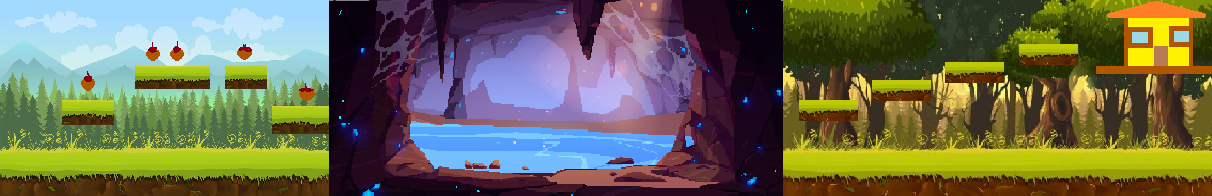
\includegraphics[width=13cm]{Modelo, juego.png}
\centering
\caption{Modelo de escenarios}
\label{fig:Modelo, juego}
\end{figure}


\section{Recursos}
\begin{itemize}
    \item la ardilla cuenta con tres vidas las cuales debe cuidar para pasar los tres niveles. 
    
\end{itemize}

\newpage

\section{Modalidad}
\begin{itemize}

    \item Las arañas se moverán de arriba hacia abajo.
    \item Las aguilas volarán de derecha a izquierda.
    \item La ardilla se moverá por el mundo hacia los lados y saltando evitando tocar los depredadores.
    \item El juego esta diseñado para un solo jugador.
\end{itemize}


\section{Diseño}

\subsection {Clases}

\begin{itemize}

    \item Personaje: esta clase se encarga de todos los cambios de sprites del personaje principal y de realizar el movimiento de este.
    
    - Metodos: movimiento, saltar, cambio de sprites.
    
    \item Arañas: manejo de sprites para el enemigo  y verificar si el personaje colisiona con alguna de las arañas
    
    - Metodos: movimiento, cambio de sprites y colision 
    
    \item Halcones:manejo de sprites para el enemigo y verificar si el personaje colisiona con algun halcon o con alguno de los elementos que arroje. 
    
    - Metodos: movimiento, cambio de sprites, colision halcon, colision roca. 
    
    \item plataformas: la clase se encarga de generar las plataformas por las que se mueve el personaje
    
    - Metodos: generar plataformas 
    
    \item escena-1:configurar la escena del nivel 1 del juego
    
    - Metodos: generar mapa
    
    \item escena-2:configurar la escena del nivel 2 del juego 
    
    - Metodos: generar mapa
    
    \item escena-3:configurar la escena del nivel 3 del juego
    
    - Metodos: generar mapa
    
    \item registro: manejo del ingreso del usuario y guardar su informacion
    
    - Metodos: verificar usuario, crear usuario, guardar informacion
    
\end{itemize}
\newpage

\subsection{Cronograma}
\begin{figure}[h]
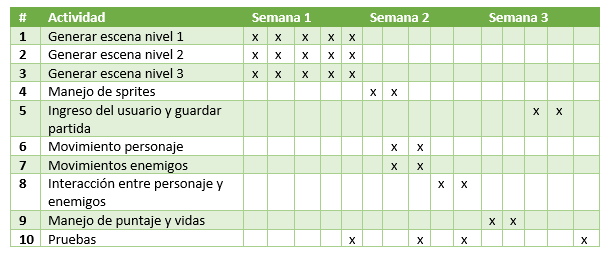
\includegraphics[width=13cm]{cronograma.PNG}
\centering
\end{figure}




\end{document}

